\documentclass[10pt]{article}
\usepackage[margin=1in]{geometry}
\usepackage{graphicx}
\usepackage{booktabs}
\usepackage{amsmath}
\usepackage[hidelinks]{hyperref}
\usepackage{microtype}
\usepackage[font=small]{caption}
\newcommand{\randomScore}{0.10}
\newcommand{\randomLevels}{7}
\newcommand{\randomGames}{6}
\newcommand{\randomFirst}{1935}
\newcommand{\frontierScore}{0.37}
\newcommand{\frontierLevels}{19}
\newcommand{\frontierGames}{12}
\newcommand{\frontierFirst}{596}
\newcommand{\undoScore}{0.38}
\newcommand{\undoLevels}{22}
\newcommand{\undoGames}{15}
\newcommand{\undoFirst}{812}
\newcommand{\totalLevels}{183}
\newcommand{\nSeeds}{3}
\newcommand{\sharereversible}{30}
\newcommand{\shareirreversible}{29}
\newcommand{\sharenoop}{40}
\newcommand{\sharefatal}{1}
\newcommand{\undoVerified}{5}
\newcommand{\invGames}{17}
\newcommand{\nStates}{59421}

\title{Undo-First Exploration: Reversibility-Aware Frontier Search for ARC-AGI-3}
\author{Sundar Shahi Thakuri\\ Independent researcher \\ \small ARC Prize 2026 Paper Track (ARC-AGI-3)}
\date{November 2026}
\begin{document}
\maketitle

\begin{abstract}
ARC-AGI-3 scores an agent by how many actions it needs to beat each level of an unseen game, squared against a human baseline. Every probing action costs, and an action that cannot be taken back can cost a reset and everything since the level started. We present \emph{undo-first exploration}, a training-free, LLM-free agent that makes reversibility the organising signal for exploration. It builds a transition graph of each level, learns online which action types can be undone and which cells are only a UI counter, probes likely-undoable actions first, and picks the next frontier by travel cost plus the expected cost of getting back. On the 25 public games, with 10{,}000 actions per game and \nSeeds{} seeds, it completes \undoLevels{} of \totalLevels{} levels (median), against \frontierLevels{} for the same explorer without the reversibility terms and \randomLevels{} for random play, and finds that \shareirreversible\% of tested transitions had no known way back. The code is attached as an offline notebook.
\end{abstract}

\section{Introduction}
ARC-AGI-3~\cite{arc3} replaces static puzzles with turn-based games on a $64{\times}64$ grid of 16 colours. Nothing is explained: the agent must discover what its actions do, what the goal is and how to reach it, level by level. It is scored by Relative Human Action Efficiency (RHAE): for each completed level, the squared ratio of the upper-median human action count to the agent's, averaged over levels and games. Frontier models scored below 1\% at launch~\cite{arc3}; the strongest public results pair large models with code at hours of compute per game~\cite{ewm}.

We ask a narrower question: how far does structure alone go, if it is the right structure? A person meeting a new game tries a move and checks whether it can be taken back: a move that can be undone is a free experiment, one that cannot is a commitment. The agent makes that distinction explicit: every tested transition is a no-op, fatal (it ended the game), reversible (a known way back exists) or not yet reversible; it learns per action type how often each class occurs, and spends its budget where experiments are cheap to undo. This is what safe reinforcement learning asks of a robot~\cite{noturningback,leavenotrace}, asked of a puzzle solver with one life per level.

The contribution is small and measurable: (i) a reversibility-aware frontier explorer with no training and no model; (ii) an online UI-mask and inverse-pair learner that makes transition graphs well defined in these games; (iii) measurements over all 25 public games of how reversible they are and what reversibility buys over the identical explorer without it.

\section{Prior work}
Rudakov et al.~\cite{graph} solved a median of 30 of 52 preview levels with a training-free graph explorer that segments frames, prioritises salient click targets and walks to the nearest untested state--action pair; an unhandled reset-inducing action trapped their official run in a loop, the failure transition classes prevent. Liew~\cite{aera} pairs a 0.5B language model with an explore--verify--plan loop (RHAE 0.21 on the public set), prefers \texttt{ACTION7} after exploratory moves, and shows that every public game falls to non-intelligent strategies, including a library crash that misreports a win; we exploit none of these. Rodionov~\cite{ewm} fully solves 15 of 25 games with an executable world model and GPT-5.5, at hours per game. Go-Explore~\cite{goexplore} returns to promising states before exploring; reversibility-aware RL~\cite{noturningback,leavenotrace} learns which actions can be undone to keep an agent safe. We bring the second idea to the first setting, with a transition graph in place of a learned estimator.

\section{Approach}
\begin{figure}[t]
\centering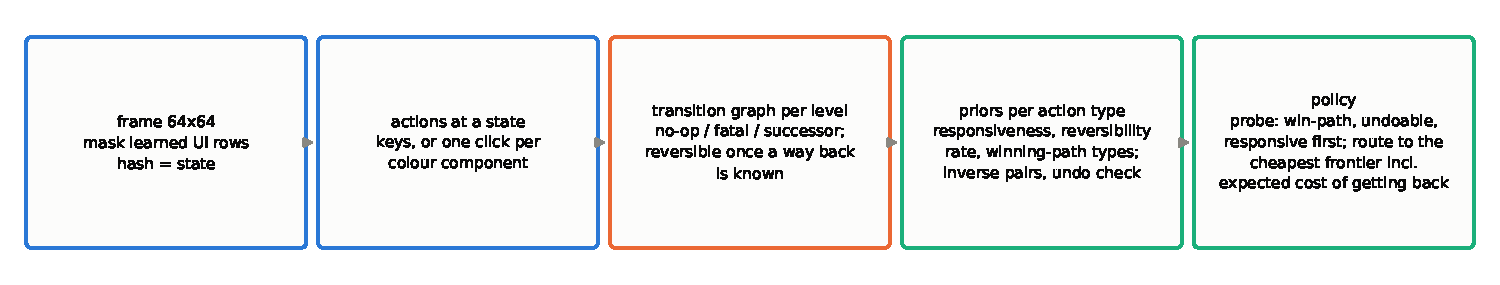
\includegraphics[width=\linewidth]{figures/fig3_method.pdf}
\caption{\label{fig:method}One step of the agent. Colour marks which part each mode uses: blue is shared by every mode, orange is the frontier explorer, green is what undo-first adds.}
\end{figure}

\paragraph{State.} The observation after an action is the last rendered frame. Games draw a step counter in an edge row that ticks as actions are spent, which would make most states unique, so an edge row (top or bottom four) that changes by at most two cells in one transition is treated as UI and zeroed before hashing; the mask is learned in the first few actions and kept for the game. A state is the hash of the masked frame.

\paragraph{Actions.} Keyboard actions are used as given. \texttt{ACTION6} is expanded into one click per connected same-colour component (largest first, at most 40, background dropped), tagged with its colour; \texttt{ACTION7} is tested like any other action. \texttt{RESET} is reserved for \texttt{GAME\_OVER} and for returning to a level start that still has untested actions.

\paragraph{Graph and classes.} Each level gets a fresh directed graph: nodes are states; an edge is a tested (state, action) with its outcome, which is a no-op (same state), fatal (\texttt{GAME\_OVER}) or a successor. A successor edge becomes \emph{reversible} the moment any tested edge leads back from the successor to the source. Three priors survive level changes, keyed by action type (action id, or clicked colour): responsiveness (share of tests that changed the state), reversibility rate (share of state changes with a known way back), and the action types on the shortest start-to-win path of earlier levels. Per game it also learns inverse pairs ($a_0$ then $a$ returns to the state two steps back) and whether \texttt{ACTION7} is a working undo.

\paragraph{Policy.} At a state with untested actions the agent tests one, ordered by winning-path membership, then (undo mode only) predicted reversibility, then responsiveness. Otherwise it plans a Dijkstra route over known edges to the cheapest frontier state and follows the cached plan until it arrives or is surprised. In undo mode an edge without a known way back costs one extra, and a frontier's cost adds $(1-p_{\mathrm{rev}})\,(1+d_{\mathrm{start}})$: the expected price of a \texttt{RESET} and a replay from the level start if the probe there cannot be undone. Fatal edges are never re-taken; after \texttt{GAME\_OVER} the agent resets; after a level is won it keeps only the priors.

\paragraph{Baselines.} \emph{random} is the Kaggle starter policy. \emph{frontier} is the identical code with the reversibility terms switched off: same mask, same responsiveness and winning-path priors, nearest frontier. The comparison isolates what reversibility adds.

\paragraph{Scoring.} The toolkit's own calculator: a level scores $\min\big((h/a)^2\cdot 100,\ 115\big)$ with resets counted in $a$, a game is the level-index-weighted mean, a run the mean over games. All runs are offline on the public \texttt{arc-agi} engine, numpy only.

\section{Results}
\begin{table}[h]
\centering\small
\begin{tabular}{lrrrrr}
\toprule
mode & score & levels (per seed) & games with a level & actions / solved level & resets \\
\midrule
random (Kaggle starter) & \randomScore & \randomLevels\ (7, 6, 7) & \randomGames/25 & 2{,}088 & -- \\
frontier, no reversibility & \frontierScore & \frontierLevels\ (18, 19, 21) & \frontierGames/25 & 644 & 27{,}112 \\
undo-first (ours) & \undoScore & \undoLevels\ (21, 22, 24) & \undoGames/25 & 812 & 20{,}048 \\
\bottomrule
\end{tabular}
\caption{\label{tab:main}25 public games, 10{,}000 actions per game, \nSeeds{} seeds. Score is the official formula (0--100), levels and games are medians over seeds out of \totalLevels{} levels, actions per solved level is the median over all solved levels, resets are summed over the three seeds.}
\end{table}

Both explorers beat random play by a wide margin (Table~\ref{tab:main}, Figure~\ref{fig:levels}). Undo-first completes \undoLevels{} levels (median) against \frontierLevels{} for the identical explorer without the reversibility terms, and reaches a first level in \undoGames{} games rather than \frontierGames{}. The gain holds on every seed but is modest, about one level in six, and it has a price: undo-first spends more actions per solved level (median 812 against 644), because it prefers probes it can take back over probes that happen to be productive. The official score does not move (\undoScore{} against \frontierScore{} out of 100). With hundreds of actions per level against human baselines of 6 to 578, RHAE is near zero for any explorer without a model of the goal; levels completed is the informative metric here.

Undo-first made 26\% fewer deliberate \texttt{RESET}s over three seeds (returns to the level start: 20{,}048 against 27{,}112; game-over resets were about equal, 7{,}743 against 7{,}938), and 51\% of the state-changing transitions it tested had a known way back by the end of a run, against 43\% for the baseline: the ordering keeps the agent in the undoable part of each level. The extra levels come mostly from two games the baseline never enters: cn04 (level 1 on every seed) and tu93 (level 2 on two seeds). Neither explorer completes a third level in any game except lp85 (5 of 8).

\paragraph{How reversible are the games?} Over all levels reached (Figure~\ref{fig:edges}), \sharenoop\% of tested transitions were no-ops, \sharereversible\% had a known way back, \shareirreversible\% had none and \sharefatal\% ended the game. The split is a property of the game: keyboard games such as re86, ka59 and cd82 are over 85\% reversible once inverse pairs are learned (\invGames{} of 25 games yielded them), while click-driven games such as r11l, lp85 and su15 are 97 to 99\% one-way. \texttt{ACTION7} was verified as a working undo in \undoVerified{} games (ar25, bp35, lf52, sk48, su15) and not in sb26, where it did not return to the previous state. Random play reaches a first level in \randomGames{} games, in line with Liew's finding that several public games fall to blind strategies; this entry has no private-set number.

\begin{figure}[t]
\centering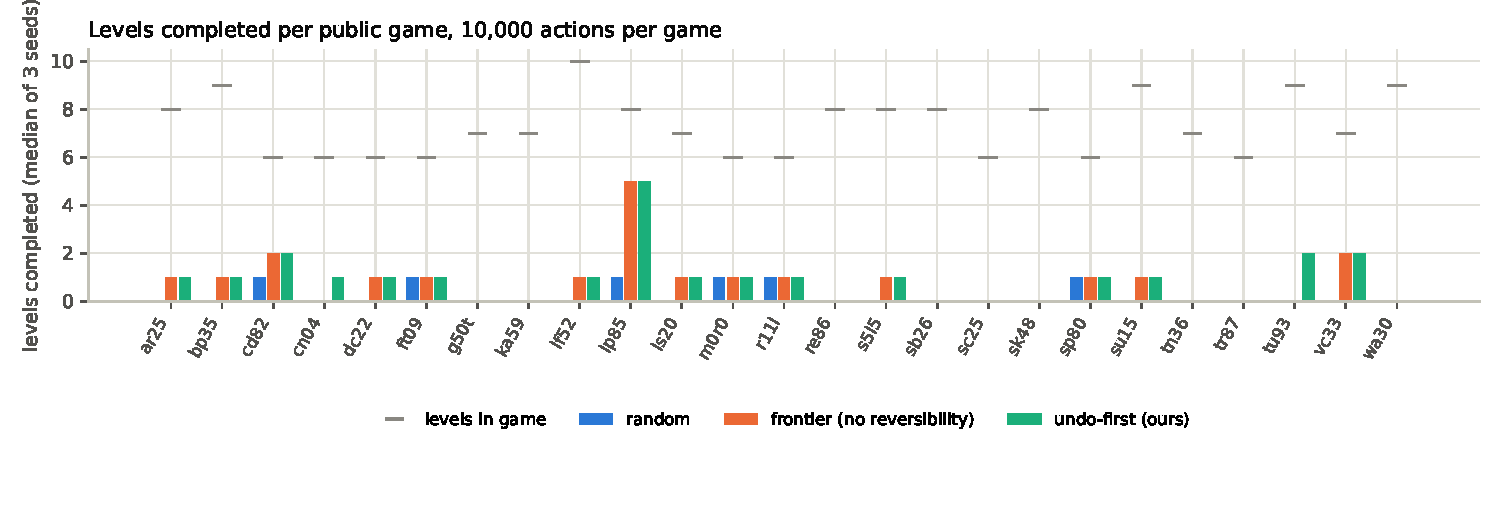
\includegraphics[width=\linewidth]{figures/fig1_levels.pdf}
\caption{\label{fig:levels}Levels completed per public game at 10{,}000 actions, median of \nSeeds{} seeds. Grey ticks mark the number of levels in each game.}
\end{figure}

\begin{figure}[t]
\centering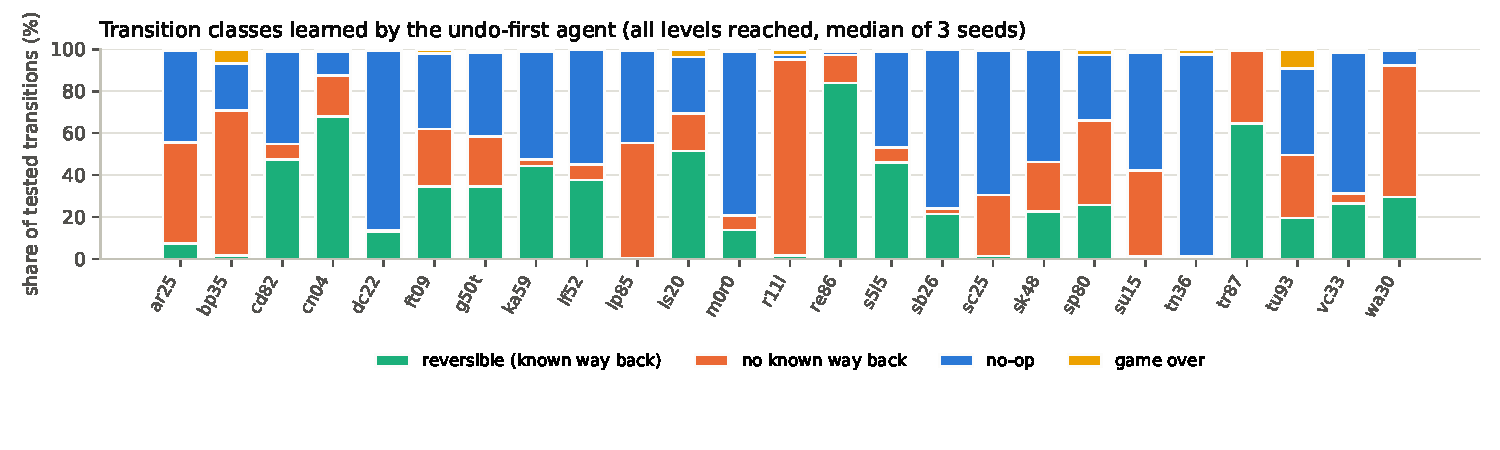
\includegraphics[width=\linewidth]{figures/fig2_edges.pdf}
\caption{\label{fig:edges}What the undo-first agent found: final class of every tested transition, all levels reached, median of \nSeeds{} seeds.}
\end{figure}

\section{Conclusion}
Reversibility is cheap to learn from a transition graph, one extra action per probe at most, and it buys a consistent but small improvement in coverage for a model-free explorer: more levels, more games entered, fewer resets. It does not buy action efficiency: RHAE rewards knowing the goal, and an agent that classifies its moves still has to guess what the level wants. The right place for an undo map is underneath a planner: a model-based agent could be held to probing only through transitions it knows how to reverse, and to spending irreversible actions only once its plan is verified. Three limitations bound the numbers: reversibility is one step deep, the UI mask is a row rule for the grid's edges, and clicks are one per colour component, so levels that need a precise cell are out of reach. The agent is a baseline others can build on, and a measurement of how much of ARC-AGI-3 can be taken back.

\paragraph{Reproducibility.} The attached notebook holds the complete agent (one file), the runner and the three-mode comparison; it runs offline in a few minutes and produces every number here. CC BY 4.0. Writing and code were produced with AI assistance (Claude Code); every number was measured by the notebook.

\begin{thebibliography}{9}
\bibitem{arc3} ARC Prize Foundation. ARC-AGI-3: A New Challenge for Frontier Agentic Intelligence. arXiv:2603.24621, 2026.
\bibitem{graph} E. Rudakov, J. Shock, B. U. Cowley. Graph-Based Exploration for ARC-AGI-3 Interactive Reasoning Tasks. arXiv:2512.24156, 2025.
\bibitem{aera} K. H. Liew. Explore Before You Solve: The Speed--Depth Trade-off in Epistemic Agents for ARC-AGI-3. arXiv:2605.25931, 2026.
\bibitem{ewm} S. Rodionov. Executable World Models for ARC-AGI-3 in the Era of Coding Agents. arXiv:2605.05138, 2026.
\bibitem{noturningback} N. Grinsztajn, J. Ferret, O. Pietquin, P. Preux, M. Geist. There Is No Turning Back: A Self-Supervised Approach for Reversibility-Aware Reinforcement Learning. NeurIPS, 2021.
\bibitem{leavenotrace} B. Eysenbach, S. Gu, J. Ibarz, S. Levine. Leave no Trace: Learning to Reset for Safe and Autonomous Reinforcement Learning. ICLR, 2018.
\bibitem{goexplore} A. Ecoffet, J. Huizinga, J. Lehman, K. O. Stanley, J. Clune. First return, then explore. Nature 590:580--586, 2021.
\bibitem{toolkit} ARC Prize Foundation. ARC-AGI Toolkit (\texttt{arc-agi} 0.9.9) and ARC-AGI-3-Agents. \url{https://github.com/arcprize/ARC-AGI}, 2026.
\end{thebibliography}
\end{document}
